% Initial version by Darian Muresan, Ph.D.
% dmuresan@stevens.edu
% Edit and adjust as needed.
\documentclass[12pt]{cornell}

% add index support
%\usepackage{imakeidx}
\usepackage{makeidx}
\usepackage{graphicx}
%\makeindex

% graphing programs
\usepackage{color}
\usepackage{psfrag}
\usepackage{verbatim}
\usepackage{fancyhdr}
%\usepackage{titlesec}
\usepackage{fancyvrb} 
% hyperlink programs
%\usepackage{url}

% Does not work with LaTeX=>PDF
\usepackage[pdfmark, 
breaklinks=true, 
colorlinks=true,
citecolor=blue,
linkcolor=blue,
menucolor=black,
pagecolor=black,
urlcolor=blue
]{hyperref} % links in pdf

%\usepackage[colorlinks]{hyperref} % links in dvi
\usepackage{listings}
\usepackage{amsfonts} 
\usepackage{amssymb} 
%\usepackage{tabto}

\usepackage{tabularx,colortbl}
\usepackage[chapter]{algorithm} 
\usepackage{algorithmic} 
\usepackage{blindtext}

\definecolor{DarkGreen}{rgb}{0,0.6,0}
\definecolor{mygreen}{rgb}{0,0.6,0}
\definecolor{mygray}{rgb}{0.5,0.5,0.5}
\definecolor{mymauve}{rgb}{0.58,0,0.82}

\usepackage{tocloft}
\usepackage{amsmath}
\usepackage{tcolorbox}
\usepackage{enumitem}
\usepackage{longtable}
%\usepackage{textcomp}
\usepackage{txfonts}
\usepackage{pstool}
\usepackage{minted}

%part for \part titles
%chap for \chapter titles
%sec for \section titles
%subsec for \subsection titles
%subsubsec for \subsubsection titles
%para for \paragraph titles
%subpara for \subparagraph titles
%fig for figure \caption titles
%subfig for subfigure \caption titles
%tab for table \caption titles
%subtab for subtable \caption titles


% update chapter number spacing
\setlength{\cftchapnumwidth}{2em}
\setlength{\cftsecnumwidth}{2.5em}
\setlength{\cftsubsecnumwidth}{3.5em}
\setlength{\cftsubsubsecnumwidth}{4.5em}

\addtolength{\cftsecindent}{0.5em}
\addtolength{\cftsubsecindent}{0.5em}
\addtolength{\cftsubsubsecindent}{0.5em}

%\titlespacing*{\chapter}{0pt}{-50pt}{20pt}
%\titleformat{\chapter}[display]{\normalfont\huge\bfseries}{\chaptertitlename\ 
%\thechapter}{20pt}{\Huge}
%\pagestyle{fancy}
%\pagestyle{cornell}
%
%\rhead{F054-021-0172}
%\chead{Nonlinear Enhancement of Visual Target Detection (AF05-T021)}
%\lhead{GSTI}
%\lfoot{\scriptsize Use or disclosure of data on this page is subject
%to the restriction on the title page of this proposal.}
%\cfoot{}
%\rfoot{\thepage}

\newfont{\Bp}{msbm10}
\newfont{\BpBig}{msbm10 scaled\magstep2}
\newfont{\Sc}{eusm10}
\newfont{\ScBig}{eusm10 scaled\magstep3}
\newfont{\Fr}{eufm10}
\newfont{\FrBig}{eufm10 scaled\magstep1}

% some commands:
\newcommand{\dxi}{{\tt m\_xDeltaInput}}
\newcommand{\dyi}{{\tt m\_yDeltaInput}}
\newcommand{\dci}{{\tt m\_cDeltaInput}}
\newcommand{\dxo}{{\tt m\_xDeltaOutput}}
\newcommand{\dyo}{{\tt m\_yDeltaOutput}}
\newcommand{\dco}{{\tt m\_cDeltaOutput}}
\newcommand{\ttf}[1]{{\tt #1}}
\newcommand{\tbl}[2]{{\begin{tabular}{c} #1 \\ #2 \end{tabular}}}

\newcommand{\urltwo}[2]{\mbox{\href{#1}{\tt #2}}}
\newcommand{\qnorm}[1]{\|#1\|_{\bQ}}
\newcommand{\qdot}[2]{\lrb #1, #2 \rrb_{\bQ}}
\newcommand{\kdot}[2]{\lrb #1, #2 \rrb_{\bf k}}
\newcommand{\tdot}[2]{\lrb #1, #2 \rrb}
\newcommand{\mydiff}[2]{\lrb #1 - #2 \rrb}
\newcommand{\lena}{\textit{lena}}
\newcommand{\barb}{\textit{barbara}}
\newcommand{\boat}{\textit{boat}}
\newcommand{\leaves}{\textit{leaves}}
\newcommand{\rings}{\textit{rings}}
\newcommand{\treg}{\textit{train region}}
\newcommand{\dreg}{\textit{denoise region}}
\newcommand{\oreg}{\textit{overlap region}}
\newcommand{\sil}{\sigma_l^2}
\newcommand{\sn}{\sigma^2}
\newcommand{\bn}{{\mbox{\bf \FrBig N}}}
\newcommand{\n}{\mbox{\Fr N}}
%\newcommand{\bn}{\bf N}
%\newcommand{\n}{N}
\newcommand{\bY}{\textbf{Y}}
\newcommand{\bX}{\textbf{X}}
\newcommand{\bb}{\textbf{b}}
\newcommand{\bu}{\textbf{u}}
\newcommand{\bv}{\textbf{v}}
\newcommand{\by}{\textbf{y}}
\newcommand{\bx}{\textbf{x}}
\newcommand{\be}{\textbf{e}}
\newcommand{\bz}{\textbf{z}}
\newcommand{\bs}{\textbf{s}}
\newcommand{\bw}{\textbf{w}}
\newcommand{\bQ}{\textbf{Q}}
\newcommand{\bphi}{\textbf{$\phi$}}
\newcommand{\lsb}{\left[}
\newcommand{\rsb}{\right]}
\newcommand{\lrb}{\left(}
\newcommand{\rrb}{\right)}
\newcommand{\lcb}{\left\{}
\newcommand{\rcb}{\right\}}
\newcommand{\R}{\mbox{\BpBig R}}
\newcommand{\F}{{\cal F}}
\newcommand{\Fk}{\mbox{\Sc F}}
\newcommand{\bQF}{\textbf{Q}_{\mbox{\Sc F}}}
\newcommand{\N}{{\cal N}}
\newcommand{\xlz}{X_l(z)}
\newcommand{\xhz}{X_h(z)}
\newcommand{\xz}{X(z)}
\newcommand{\pr}{ perfect reconstruction }
\newcommand{\smb}{Smith-Barnwell }
\newcommand{\xw}{X(e^{j\omega})}
\newcommand{\xmw}{X(-e^{j\omega})}
\newcommand{\dw}{D(e^{j\omega})}
\newcommand{\dmw}{D(-e^{j\omega})}
\newcommand{\ew}{E(e^{j\omega})}
\newcommand{\emw}{E(-e^{j\omega})}
\newcommand{\fw}{F_0(e^{j\omega})}
\newcommand{\fmw}{F_0(-e^{j\omega})}
\newcommand{\hoz}{H_1(z)}
\newcommand{\hzz}{H_0(z)}
\newcommand{\goz}{G_1(z)}
\newcommand{\gzz}{G_0(z)}
\newcommand{\hzw}{H_{0}(e^{j\omega})}
\newcommand{\hzmw}{H_{0}(-e^{j\omega})}
\newcommand{\hzcw}{H_{0}(e^{-j\omega})}
\newcommand{\how}{H_1(e^{j\omega})}
\newcommand{\homw}{H_1(-e^{j\omega})}
\newcommand{\gzw}{G_0(e^{j\omega})}
\newcommand{\gzmw}{G_0(-e^{j\omega})}
\newcommand{\gow}{G_1(e^{j\omega})}
\newcommand{\gomw}{G_1(-e^{j\omega})}
\newcommand{\wl}{e^{-jwL}}
\newcommand{\aqua}{\textit{AQua with OR }}
\newtheorem{theorem}{Theorem}
\newtheorem{lemma}{Lemma}
\newtheorem{corollary}{Corollary}
\newtheorem{claim}{Claim}
\newtheorem{definition}{Definition}
\newenvironment{proof}{\noindent{\em Proof.}}{\ \hfill Q.E.D.}
%\newtheorem{moduleCount}{L}
\newcommand*{\labelfile}[1]{%
  \label{file:#1}%
}

% Use this to label requirements, use cases, user stories, etc.
% This is where we can add different spellings for different types of 
% requirements, use cases, user stories, etc.
% \newtheorem{requirementKind}{Requirement Spelling}
\newtheorem{reqkFunctional}{Functional Requirement}
\newtheorem{reqkQuality}{Quality Requirement}
\newtheorem{reqkConstraint}{Constraint Requirement}
\newtheorem{reqkInterface}{Interface Requirement}
\newtheorem{reqkBusiness}{Business Requirement}
% Use cases
\newtheorem{useCase}{Use Case}
% User story
\newtheorem{userStory}{User Story}

% command for adding a version to the document
\newcommand{\VERSION}{Version 0.0.0}

% Family -- enter the name of the family that it belongs to: Chapter, Figure, Table, etc.
% Name -- name of the family member: file name, table name, etc.
\newcommand{\FamilyName}[2]{\hyperref[#1::#2]{#2}\index{#2}\xspace}
% Family -- same as above
% Name -- same as above
% Reference -- shorthand for the 'Name'.  It will show as Reference_NameID
% Kind -- underscore(_), space, or dash (-)
\newcommand{\FamilyNameReferenceKind}[4]{\hyperref[#1::#2]{$#3#4{\ref*{#1::#2}}$}}
% newcommand{Family,Label}
\newcommand{\FamilyLabel}[2]{\label{#1::#2}}


% for use cases
\newcommand{\UseCaseLabel}[1]{\FamilyLabel{UseCase}{#1}}
\newcommand{\UseCaseName}[1]{\FamilyName{UseCase}{#1}}
\newcommand{\UseCaseReference}[1]{\FamilyNameReferenceKind{UseCase}{#1}{UC}{_}}
% UseCase name with stacked reference
\newcommand{\UseCaseNameWSReference}[1]{\begin{tabular}{c}\UseCaseName{#1} \\ (\UseCaseReference{#1}) \end{tabular}}
% UseCase name with inline reference
\newcommand{\UseCaseNameWIReference}[1]{\UseCaseName{#1} (\UseCaseReference{#1})}

% for chapters
\newcommand{\ChapterName}[1]{\FamilyName{Chapter}{#1}}
\newcommand{\ChapterLabel}[1]{\FamilyLabel{Chapter}{#1}}
\newcommand{\ChapterReference}[1]{\FamilyNameReferenceKind{Chapter}{#1}{Chapter}{\mbox{ }}}
% Chapter name with inline (WI) reference 
\newcommand{\ChapterNameWIReference}[1]{\ChapterName{#1} (\ChapterReference{#1})}

% for figures
\newcommand{\FigureName}[1]{\FamilyName{Figure}{#1}}
\newcommand{\FigureLabel}[1]{\FamilyLabel{Figure}{#1}}
\newcommand{\FigureReference}[1]{\FamilyNameReferenceKind{Figure}{#1}{Figure}{\mbox{ }}}
% Figure name with stacked (WS) reference
\newcommand{\FigureNameWSReference}[1]{\begin{tabular}{c}\FigureName{#1} \\ (\FigureReference{#1}) \end{tabular}}
% Figure name with inline (WI) reference 
\newcommand{\FigureNameWIReference}[1]{\FigureName{#1} (\FigureReference{#1})}

% for tables
\newcommand{\TableName}[1]{\FamilyName{Table}{#1}}
\newcommand{\TableLabel}[1]{\FamilyLabel{Table}{#1}}
\newcommand{\TableReference}[1]{\FamilyNameReferenceKind{Table}{#1}{Table}{\mbox{ }}}

% for requirements
% RequirementLabel[Kind][Label]
\newcommand{\RequirementLabel}[2]{\FamilyLabel{#1}{#2}}
\newcommand{\RequirementName}[2]{\FamilyName{#1}{#2}}
\newcommand{\RequirementReference}[2]{\FamilyNameReferenceKind{#1}{#2}{#1}{_}}
% Requirements name with stacked (WS) reference
\newcommand{\RequirementNameWSReference}[2]{\begin{tabular}{c}\RequirementName{#1}{#2} \\ (\RequirementReference{#1}{#2}) \end{tabular}}
% Requirements name with inline (WI) reference 
\newcommand{\RequirementNameWIReference}[2]{\RequirementName{#1}{#1} (\RequirementReference{#1}{#2})}

% for requirements
% RequirementLabel[Kind][Label]
\newcommand{\UserStoryLabel}[2]{\FamilyLabel{#1}{#2}}
\newcommand{\UserStoryName}[2]{\FamilyName{#1}{#2}}
\newcommand{\UserStoryReference}[2]{\FamilyNameReferenceKind{#1}{#2}{R}{_}}
% Requirements name with stacked (WS) reference
\newcommand{\UserStoryNameWSReference}[2]{\begin{tabular}{c}\RequirementName{#1}{#2} \\ (\RequirementReference{#1}{#2}) \end{tabular}}
% Requirements name with inline (WI) reference 
\newcommand{\UserStoryNameWIReference}[2]{\RequirementName{#1}{#1} (\RequirementReference{#1}{#2})}



\lstset{ %
  backgroundcolor=\color{white},   % choose the background color; you must add \usepackage{color} or \usepackage{xcolor}
  basicstyle=\footnotesize,        % the size of the fonts that are used for the code
  breakatwhitespace=false,         % sets if automatic breaks should only happen at whitespace
  breaklines=true,                 % sets automatic line breaking
  captionpos=b,                    % sets the caption-position to bottom
  commentstyle=\color{DarkGreen},    % comment style
  deletekeywords={...},            % if you want to delete keywords from the given language
  escapeinside={\%*}{*)},          % if you want to add LaTeX within your code
  extendedchars=true,              % lets you use non-ASCII characters; for 8-bits encodings only, does not work with UTF-8
  %frame=single,                   % adds a frame around the code
  keepspaces=true,                 % keeps spaces in text, useful for keeping indentation of code (possibly needs columns=flexible)
  keywordstyle=\color{blue},       % keyword style
  language=C++,                    % the language of the code
  morekeywords={*,...},            % if you want to add more keywords to the set
  numbers=left,                    % where to put the line-numbers; possible values are (none, left, right)
  numbersep=5pt,                   % how far the line-numbers are from the code
  numberstyle=\tiny\color{mygray}, % the style that is used for the line-numbers
  rulecolor=\color{black},         % if not set, the frame-color may be changed on line-breaks within not-black text (e.g. comments (green here))
  showspaces=false,                % show spaces everywhere adding particular underscores; it overrides 'showstringspaces'
  showstringspaces=false,          % underline spaces within strings only
  showtabs=false,                  % show tabs within strings adding particular underscores
  stepnumber=1,                    % the step between two line-numbers. If it's 1, each line will be numbered
  stringstyle=\color{mymauve}     % string literal style
  %tabsize=2,                      % sets default tabsize to 2 spaces
  %caption=\lstname                % show the filename of files included with \lstinputlisting; also try caption instead of title
}


% Uncomment draftcopy to get the word DRAFT boldly across the first page
%   By the way, xdvi won't show it but it will come out when you print
%\usepackage[light,all]{draftcopy}		% DRAFT on first page
%\draftcopySetGrey{.97}
%\draftcopyName{Confidential}{150}
%\draftcopFirstPage{1}

% Uncomment drafthead to get the date and DRAFT in the header of pages
% that are normallly numbered on the top, pages 2-n of each chapter for example
% This doesn't work with centered page numbers: \pagestyle{cornellc}
%\usepackage{drafthead}

% glossaries to organize the document glossary
%\usepackage[toc,chapter,numberedchapter = autolabel]{glossaries}
\usepackage{glossaries}

% glossary creation
\newglossaryentry{must}
{	name={MustHave},
	description={This defines the first highest priority requirement.
	All of the tasks, requirements, or anything that is marked this way are
	build in the current version}
}

\newglossaryentry{should}
{	name={ShouldHave},
	description={This defines the second highest priority requirement. The system should implement 
	all of the tasks, requirements, or anything that is marked this way, but if 
	resources are limited, it can be left out of the current version.
	Build in next version}
}

\newglossaryentry{could}
{	name={CouldHave},
	description={This defines the third highest priority requirement.The system could implement 
	all of the tasks, requirements, or anything that is marked this way, but if 
	resources are limited, it can be left out of the current and next version.
	Build in two versions from now}
}

\newglossaryentry{would}
{	name={WouldHave},
	description={This defines the lowest priority requirement.  The system would like to implement 
all of the tasks, requirements, or anything that is marked this way, but only
if resources are available. It can be left out of all future versions}
}

%\makeglossaries
\makenoidxglossaries
\makeindex

% Including selective chapters:
% use this to selectively process chapters, etc.  Put a % in front of
% the sections that you don't want done this time.  Includes are
% used instead of \input so that LaTeX will keep track of chapters and
% pages without processing everything.  Don't let any spaces creep in
% around the words or it will not work!

\includeonly{
prologue,
itIntroduction,
itKanbanSetup,
itPasswords,
itHosts,
itAppendix,
itLinuxCommands,
itProjectProposal,
itAWSDeployment,
itLaTeXDocker,
itBugzillaDocker,
itOverleafDocker,
itDomainNames
}


\begin{document}

\pagenumbering{roman}
\singlespacing
% File: prologue.tex
% Thesis prologue:  Title page, acknowledgements, table of contents,
% list of figures, and list of tables.
%
% this file is to be \include'd after the \begin{document}

% Cornell-style title page
\begin{titlepage}
        \title{SSW 590 - DevOps Configuration}
        \author{Tamara Gonzalez Ibarra, Sydney Winstead, Michelle Elias Flores\\ Stevens.edu }
        \conferraldate{}{\today} \maketitle
\end{titlepage}

% Copyright page
%\begin{copyrightpage}
\makecopyright
%\end{copyrightpage}

% Abstract: the abstract body is pulled from the file abstract.tex;
%  the title is pulled from the \title command in the titlepage section
\begin{abstract}
        %\makeabstitle
        \input abstract      % puts the abstract file here
\end{abstract}

% Biographical information pulled from file bio.tex
%\begin{biosketch} \input bio \end{biosketch}

% Dedication (optional):  pulls information from file dedication.tex
%\begin{dedication} 
%\input dedicate 
%\end{dedication}

% Acknowledgements:  pulls information from file acknow
%\begin{acknowledgements} \input acknow \end{acknowledgements}

% Table of contents
\contentspage

% If you have no tables or figures put a % in front of the list page line
% List of tables
\tablelistpage

% List of figures
\figurelistpage

\setcounter{page}{1}        % set page counter
\pagenumbering{arabic}      % set page number style
\pagestyle{fancy}         % top right page numbers
%\pagestyle{cornell}
%\pagestyle{cornellc}       % centered page numbers, disables drafthead

\renewcommand{\chaptermark}[1]{\markboth{#1}{}}
\renewcommand{\sectionmark}[1]{\markright{#1}{}}

\fancyhead{} % clear all fields

\lhead{Chapter \thechapter}
%\lhead{\thechapter}
\chead{\leftmark}
\rhead{\thepage}


\lfoot{Chapter \thechapter}
\cfoot{\copyright Stevens -- \today \mbox{} -- Do Not Distribute!}
\rfoot{\thepage}

\renewcommand{\headrulewidth}{0.4pt}
\renewcommand{\footrulewidth}{0.4pt}

%\rhead{F054-021-0172}
%\chead{Nonlinear Enhancement of Visual Target Detection (AF05-T021)}
%\lhead{GSTI}
%\lfoot{\scriptsize Use or disclosure of data on this page is subject
%to the restriction on the title page of this proposal.}
%\cfoot{}
%\rfoot{\thepage}


\singlespacing
\chapter{Introduction \\
\small{\textit{-- Tamara Gonzalez Ibarra, Michelle Elias Flores, Sydney Winstead}}
\index{introduction} 
\index{Chapter!Introduction}
\label{Chapter::Introduction}}

 
This document has been prepared using Overleaf. The purpose of this document is not only to complete assignments for SSW 590, but also to gain further experience in using the platform.

\section{About The Team}

\subsection{Tamara}
My name is Tamara Gonzalez Ibarra, but you can call me Tamy! I am a 4/4 Software Engineering major that is passionate about open-source projects, and my favorite programming languages are Python and Rust. Outside of class, I love being involved on campus with clubs such as LAA, SHPE, and IEEE. I am excited to learn more about DevOps in this course and gain hands-on experience in working with Docker and other platforms. 

\subsection{Sydney}
I'm Sydney Winstead, a senior software engineering student. Some random things I like are Python, Godot, and Dnb music. I've had some experience with Kanban Boards (Trello) and with Linux but that is as far as my DevOps knowledge currently goes. Looking forward to learning!

\subsection{Michelle}
My name is Michelle Elias Flores (she/her) and I am a senior Computer Science major interested in studying DevOps to learn more about how different Agile processes work together. My favorite programming langauges are Python and PL/SQL and I am excited to work with Docker.
\chapter{Kanban Setup}
\label{Chapter::KanbanSetup}
\index{Kanban Setup}
\index{Chapter!Kanban Setup}

\begin{flushleft}
\small{\textit{-- Tamara Gonzalez Ibarra}}
\end{flushleft}

In this chapter, I describe the steps I followed to set up a Kanban board with my group members in Trello. 
The purpose of the Kanban setup is to create a clear and visual workflow that helps manage tasks and track progress effectively for agile projects. 

\section{Creating the Board}
\begin{enumerate}
    \item Logged into Trello with my account.
    \item Clicked on \texttt{Create new board}.
    \item Named the board \textit{Kanban Board}, used a Kanban Board template, and selected a background for better visualization.
\end{enumerate}

\section{Setting Up Lists}
\begin{enumerate}
    \item Created the following lists to represent the workflow:
    \begin{itemize}
        \item \textbf{Backlog} – ideas and tasks that still need to be planned or refined.
        \item \textbf{Design} – tasks related to planning and designing before implementation.
        \item \textbf{To Do} – tasks that need to be started.
        \item \textbf{Doing} – tasks that are currently in progress.
        \item \textbf{Code Review} – tasks that are finished but require peer review before proceeding.
        \item \textbf{Testing} – tasks that have passed review and need to be tested for quality assurance.
        \item \textbf{Done} – completed tasks.
    \end{itemize}
    \item Ensured the lists followed a left-to-right order.
\end{enumerate}

\begin{figure}[h!]
    \centering
    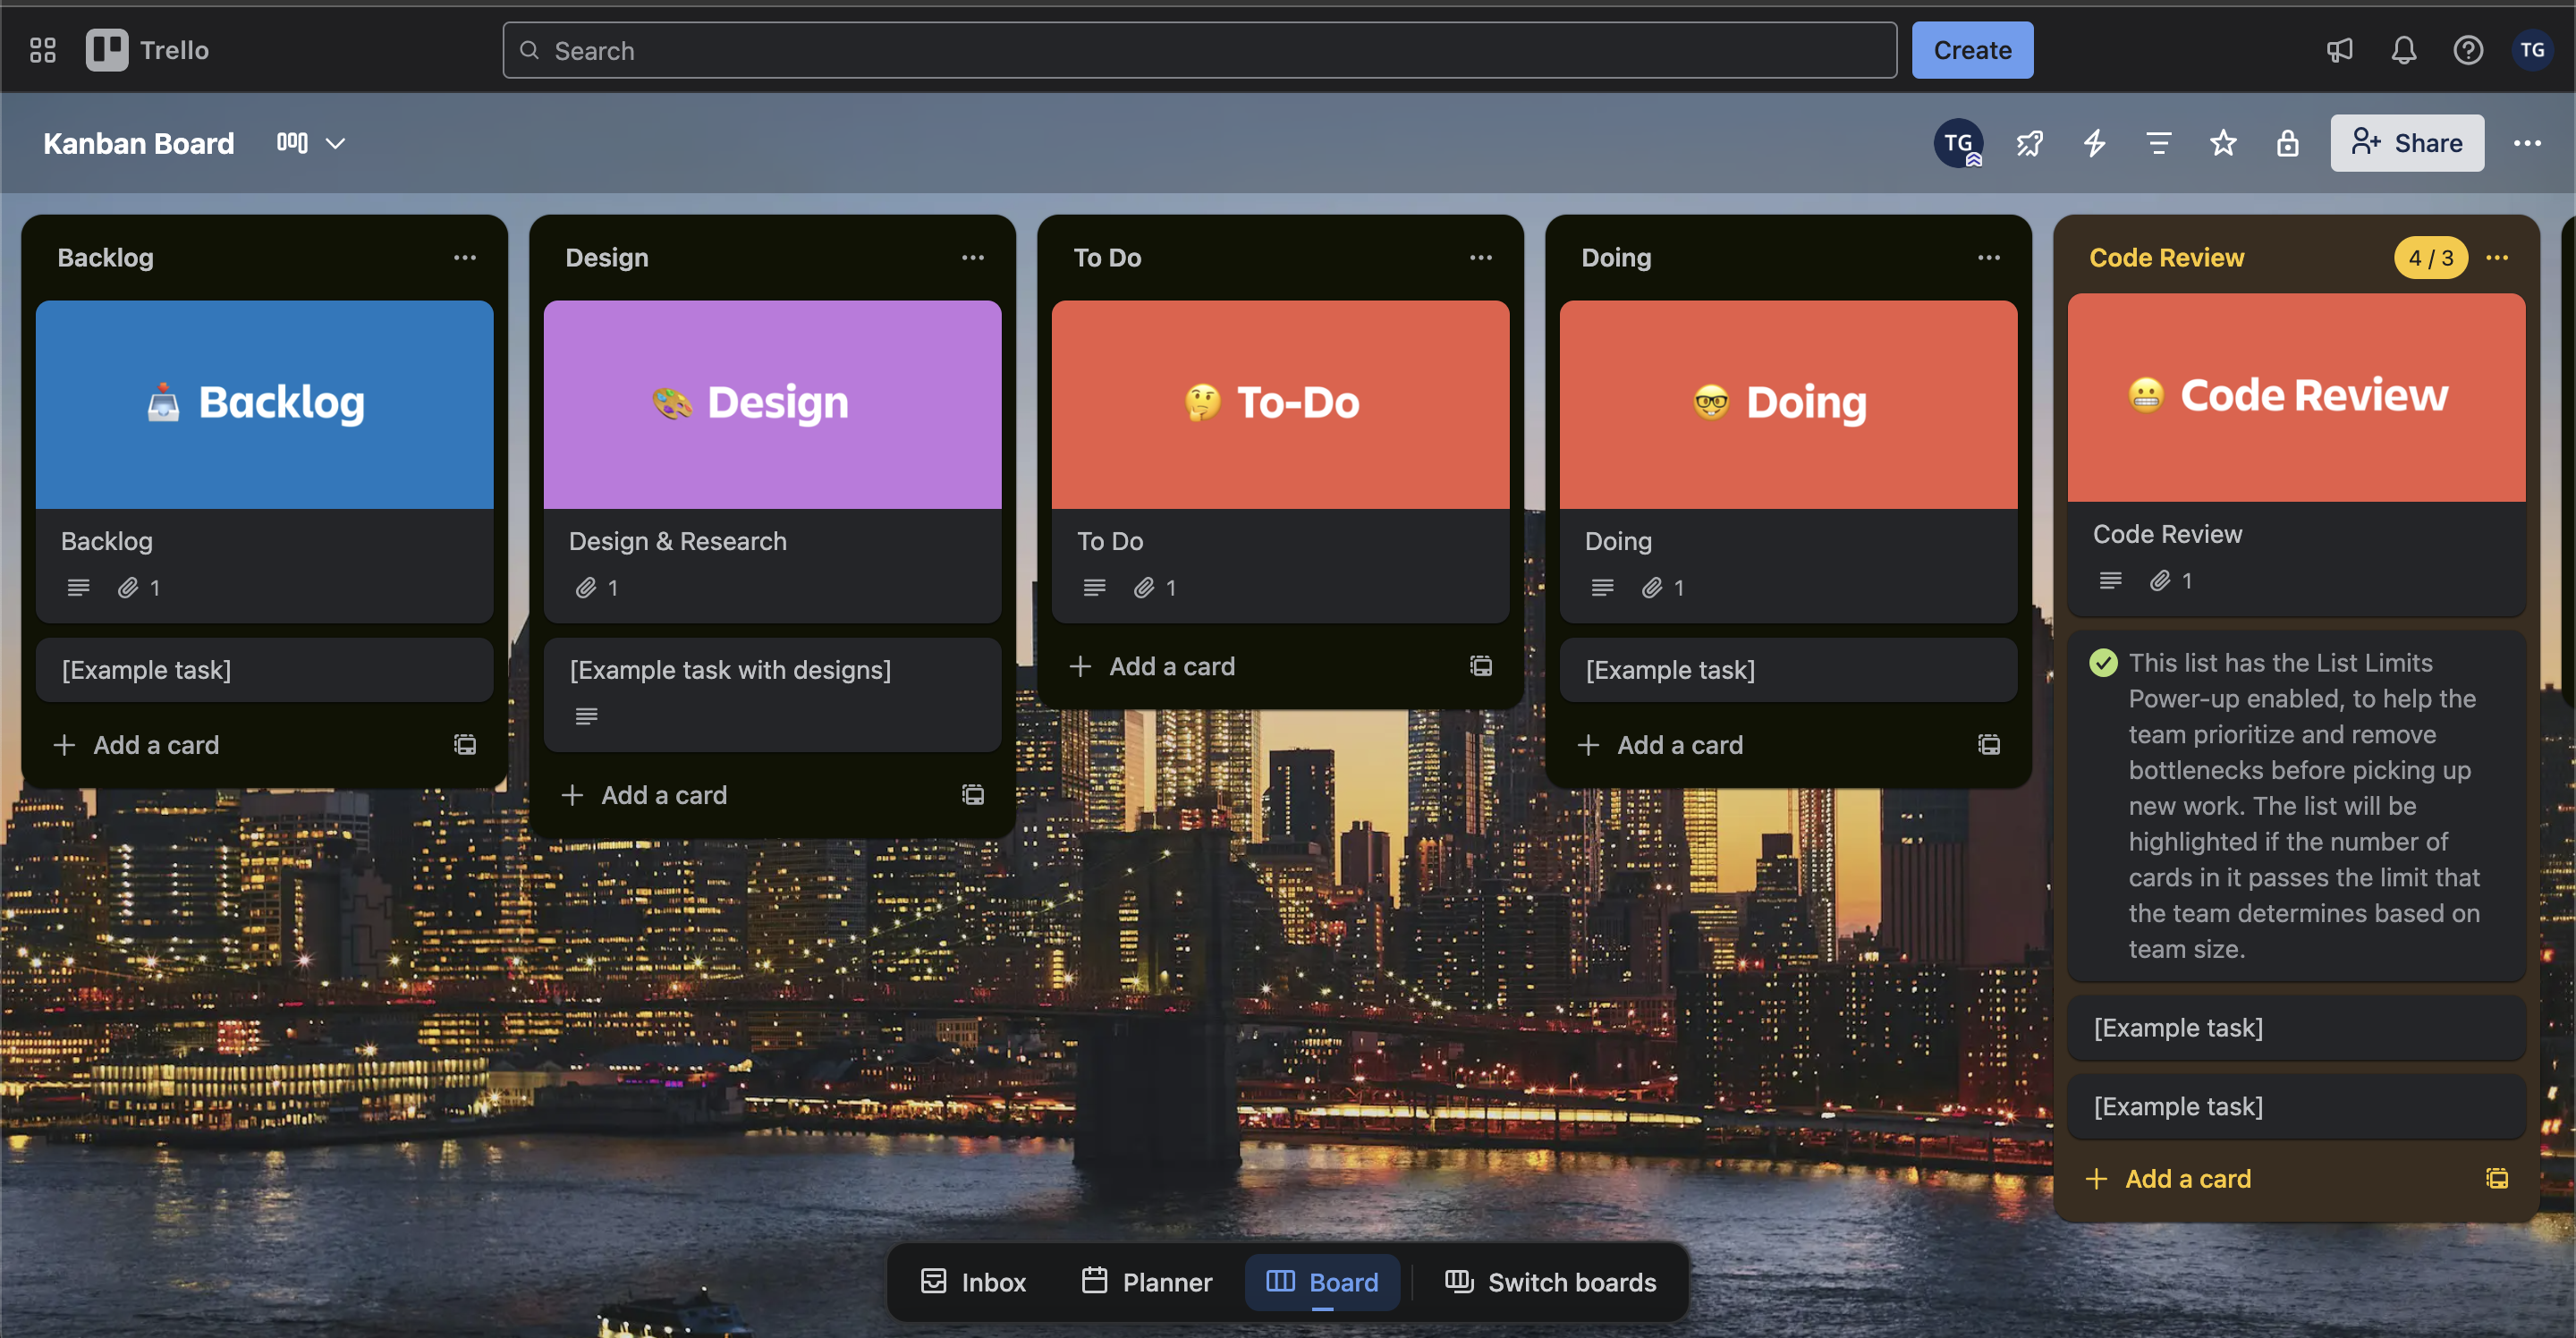
\includegraphics[width=0.8\textwidth]{kanban_board.png}
    \caption{Screenshot of the first half of the Kanban Board in Trello.}
    \label{fig:kanban_board}
    
    \vspace{0.5cm} % space between images
    
    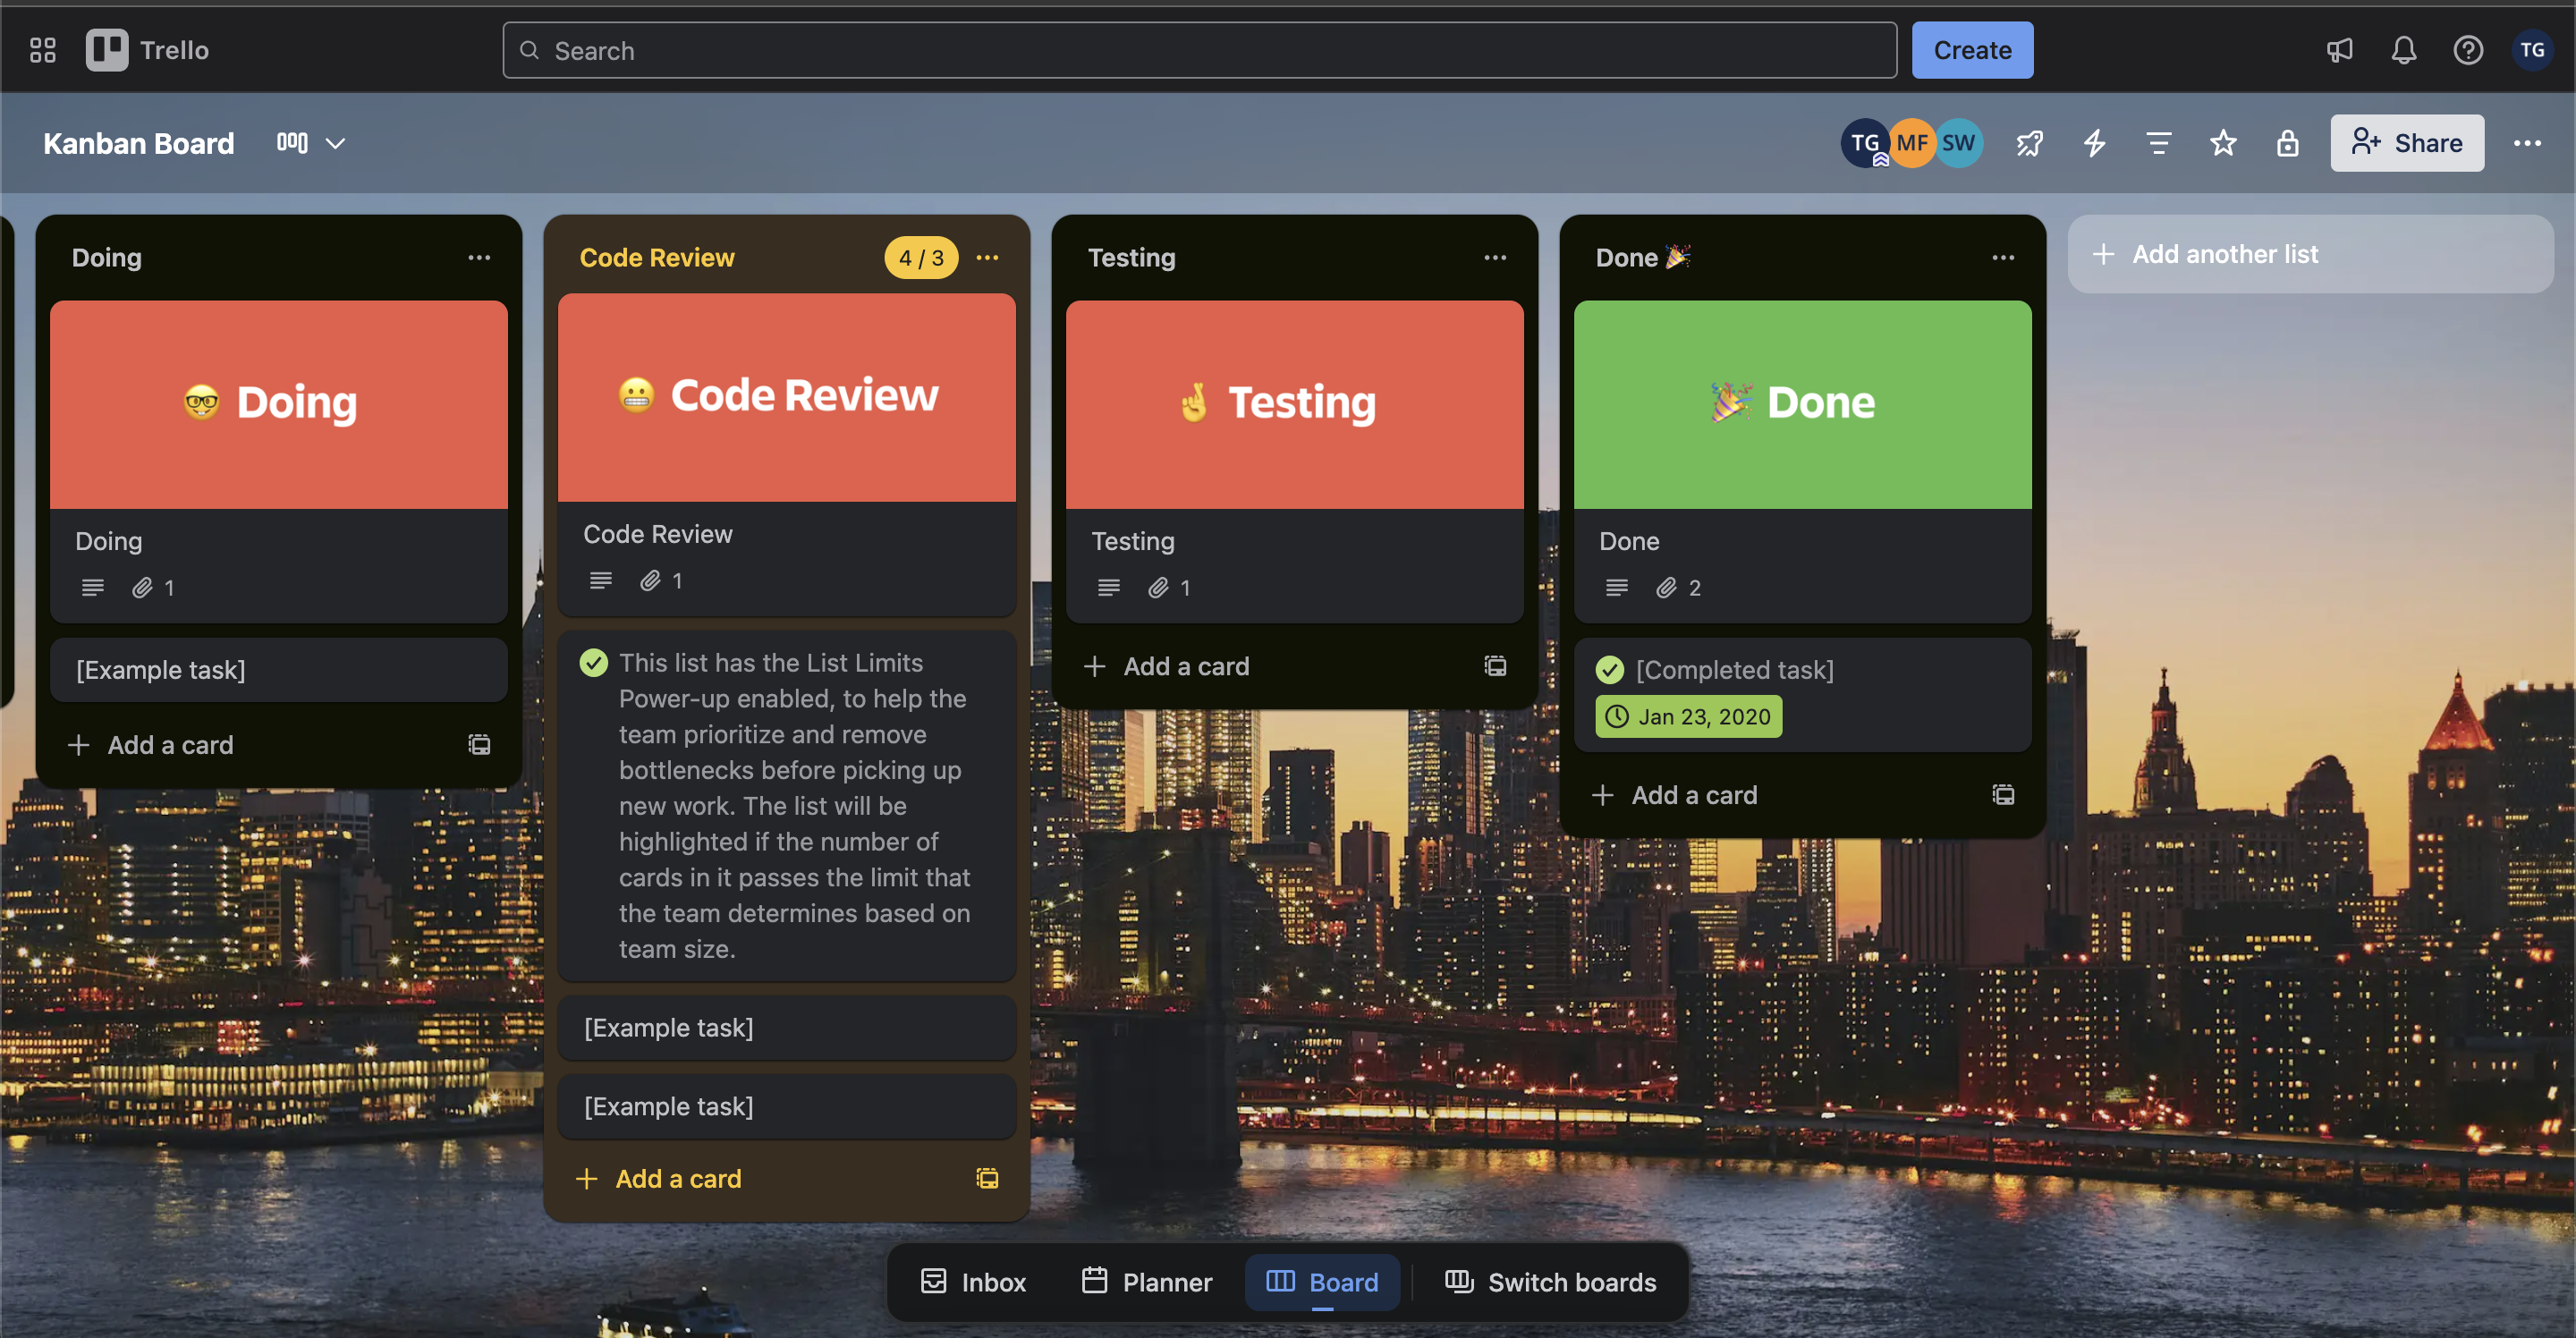
\includegraphics[width=0.8\textwidth]{kanban_board2.png}
    \caption{Screenshot of the second half of the Kanban Board in Trello.}
    \label{fig:kanban_board2}
\end{figure}

\section{Using Trello Features}
\begin{enumerate}
    \item Enabled checklists within cards to track smaller subtasks.
    \item Attached files and links directly to cards for reference.
    \item Used Trello’s built-in automation (Butler) to move cards between lists when certain conditions were met (e.g., when a task is marked complete).
\end{enumerate}

This Kanban setup provides a clear structure for a future project, making it easier to manage work, track progress, and stay organized throughout the project.

\chapter{Passwords \\
\small{\textit{-- Tamara Gonzalez Ibarra}}}
\index{Passwords} 
\index{Chapter!Passwords}
\label{Chapter::Passwords}

In this chapter, the password rules used for various users and servers in the project are displayed. 
The table below summarizes the rules for username, server, and password, along with hints to remember them. Actual passwords are not included for security reasons.

\section{Password Rules Table}

\begin{longtable}{|l|l|p{4cm}|p{4cm}|}
\hline
\textbf{User} & \textbf{Server} & \textbf{Password Rule} & \textbf{Hint} \\
\hline
\endfirsthead
\multicolumn{4}{c}%
{\tablename\ \thetable\ -- continued from previous page} \\
\hline
\textbf{User} & \textbf{Server} & \textbf{Password Rule} & \textbf{Hint} \\
\hline
\endhead
\hline \multicolumn{4}{r}{\textit{Continued on next page}} \\
\endfoot
\hline
\endlastfoot

Name1 & Server A & At least 8 characters, includes uppercase, lowercase, and a number & Think of your favorite animal and a memorable year. \\
\hline
Name2 & Server B & Minimum 10 characters, includes special character & Combine your favorite color and the number of letters in your hometown. \\
\hline
Tamy & Server C & Must include at least 1 uppercase letter, 1 lowercase letter, and 1 number; 10 characters & At least 12 characters, no repeating characters. Use the first letters of a favorite quote. \\
\hline
\textbf{Bugzilla Admin} & \textbf{167.99.121.94 (Bugzilla Docker)} & At least 10 characters; include site-specific suffix (e.g., \texttt{@bugzilla}); combine shared key with service name & Use format \texttt{<key>@bugzilla} — shared key + service name. \\
\hline
\textbf{Overleaf Admin} & \textbf{167.99.121.94 (Overleaf Docker)} & At least 10 characters; include site-specific suffix (e.g., \texttt{@overleaf}); combine shared key with service name & Use format \texttt{<key>@overleaf} — shared key + service name. \\
\hline
\textbf{Database User} & \textbf{Local Docker DBs} & At least 10 characters; include mix of upper/lowercase and a dot to indicate database scope & Use format \texttt{key.db} — same key used across both DBs with unique suffix. \\
\hline
\end{longtable}

\section{Notes on Password Rules}

All passwords are designed to be strong but memorable using personal hints. Users should avoid writing down passwords directly and instead rely on hints or a secure password manager.

\chapter{Hosts}
\label{Chapter::Hosts}
\index{Hosts}
\index{Chapter!Hosts}

\begin{flushleft}
\small{\textit{-- Tamara Gonzalez Ibarra}}
\end{flushleft}

In this chapter, the hosts that will be configured for the development environment are described. 
The table below lists the host names along with their roles and permissions.

\section{Hosts Table}

\begin{longtable}{|l|l|p{5cm}|}
\hline
\textbf{Host Name} & \textbf{Role} & \textbf{Permissions} \\
\hline
\endfirsthead
\multicolumn{3}{c}%
{\tablename\ \thetable\ -- continued from previous page} \\
\hline
\textbf{Host Name} & \textbf{Role} & \textbf{Permissions} \\
\hline
\endhead
\hline \multicolumn{3}{r}{\textit{Continued on next page}} \\
\endfoot
\hline
\endlastfoot

tamaragonzalez & Database Server & -rwxr-xr-x \\
\hline
dev-user1 & Application Server & -rwxr-x--- \\
\hline
dev-user2 & Web Server & -rw-r--r-- \\
\hline
admin & System Administrator & -rwx------ \\
\hline
backup & Backup Host & -rw------- \\
\hline
test-env & Testing Environment & -rwxrwxr-x \\
\hline
staging & Pre-Production Server & -rwxr-x--- \\
\hline
prod-main & Production Server & -rwxr----- \\
\hline

\end{longtable}

\chapter{Linux Commands \\
\small{\textit{-- Tamara Gonzalez Ibarra, Michelle Elias Flores, Sydney Winstead}}
\index{itLinuxCommands} 
\index{Chapter!itLinuxCommands}
\label{Chapter::itLinuxCommands}}

In this chapter, we have included the following screenshots of our work for the Linux Commands assignment. Completing this assignment involved practicing Linux commands for navigation, file operations, permissions, process control, networking, and scripting. 


\begin{figure}[h!]
    \centering
    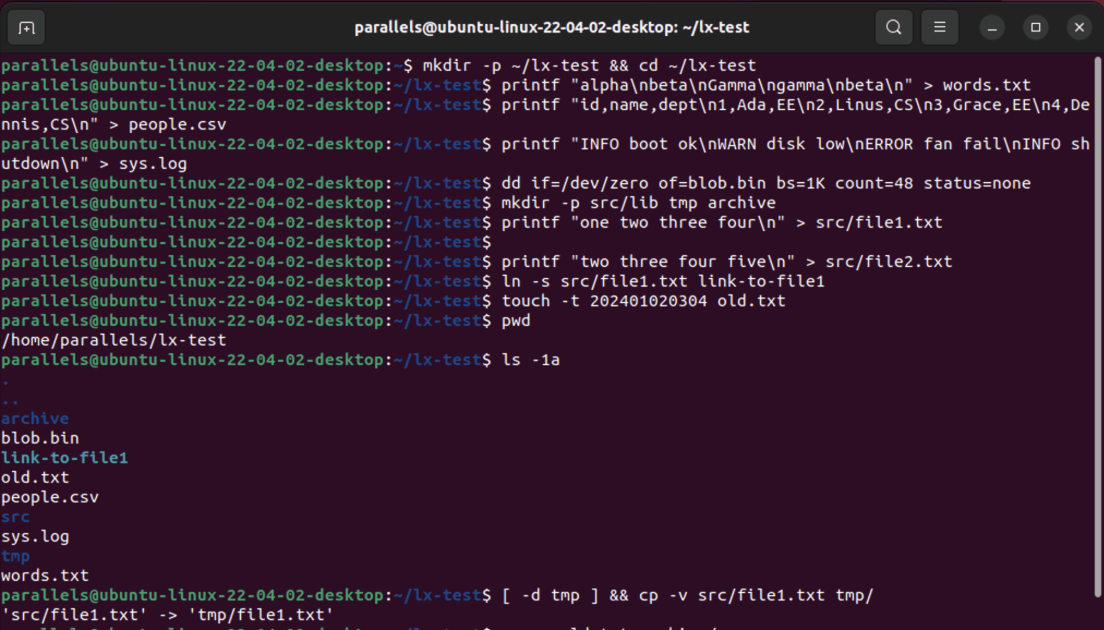
\includegraphics[width=0.8\textwidth]{linuxptA.png}
    \caption{Screenshot of the first part of A) Navigation and File Ops}
    \label{fig:problemsetA}
\end{figure}
    
\begin{figure}[h!]
    \centering
    
\includegraphics[width=0.8\textwidth]{linuxptA2.png}
    \caption{Screenshot of the second part of A) Navigation and File Ops}
    \label{fig:problemsetApt2}
\end{figure}

\begin{figure}[h!]
    \centering
    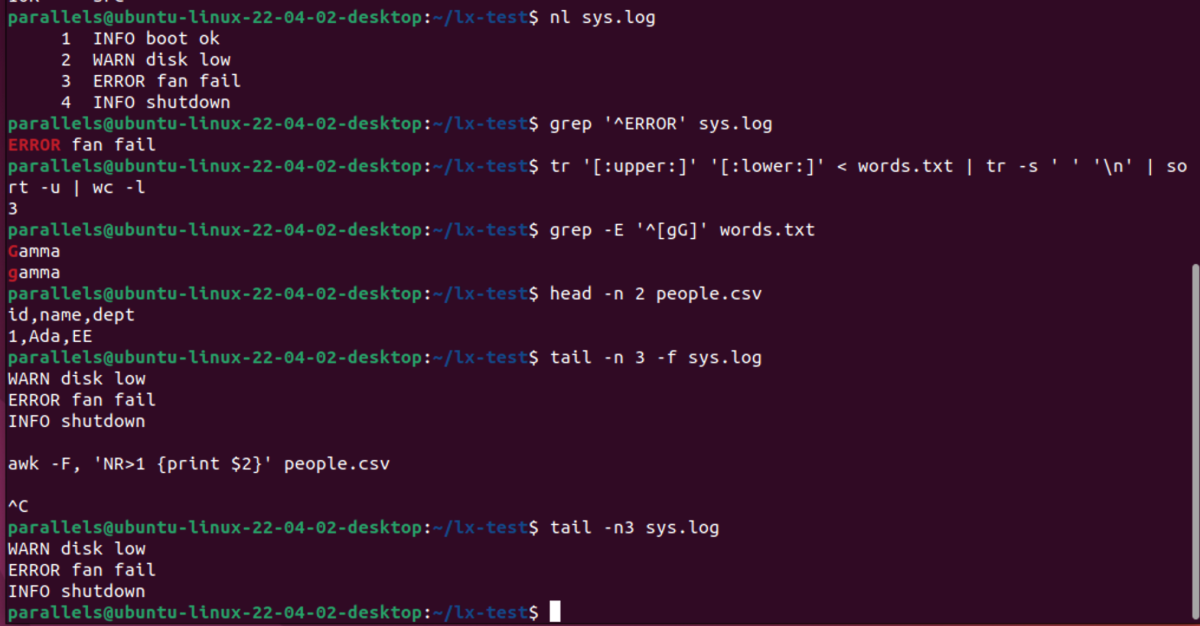
\includegraphics[width=0.8\textwidth]{linuxptB.png}
    \caption{Screenshot of Part B) Viewing and Searching}
    \label{fig:problemsetB}

\end{figure}

\begin{figure}[h!]
    \centering
    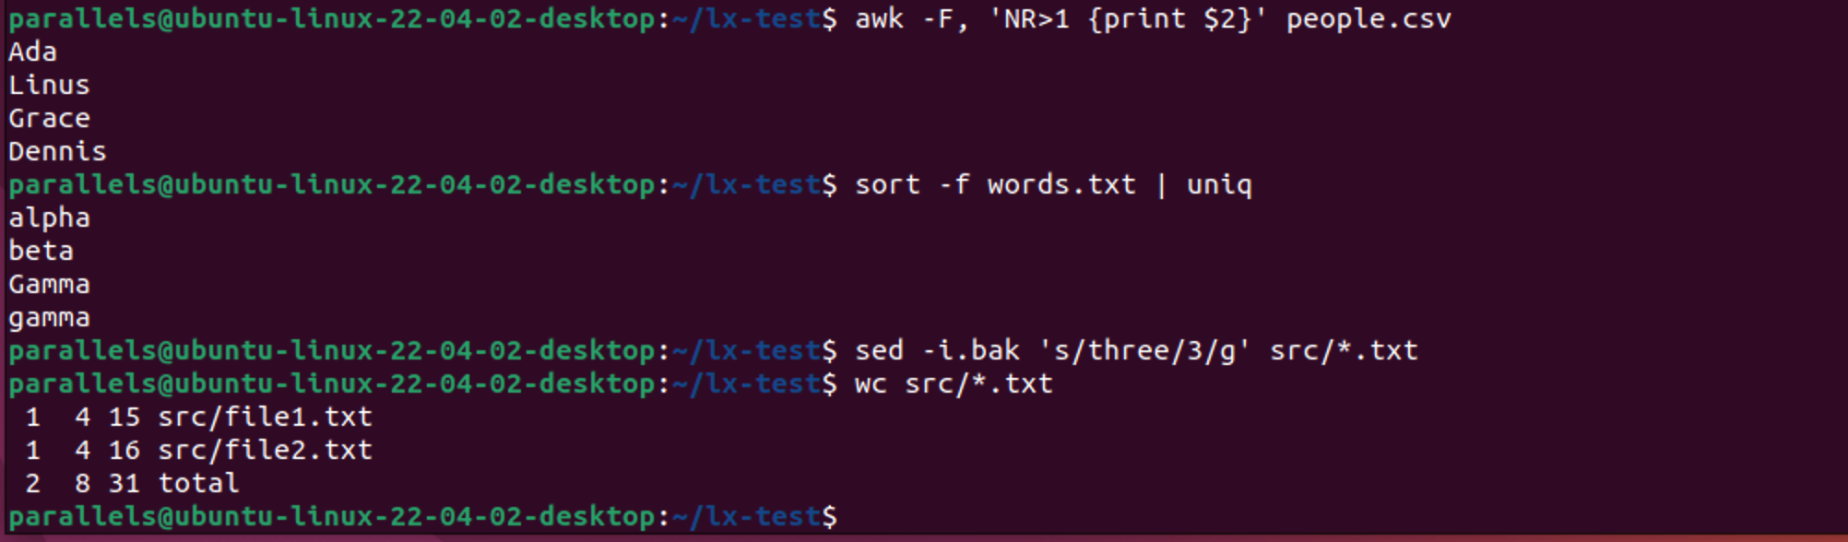
\includegraphics[width=0.8\textwidth]{linuxptC.png}
    \caption{Screenshot of Part C) Text Processing}
    \label{fig:problemsetC}
\end{figure}

\begin{figure}[h!]
    \centering
    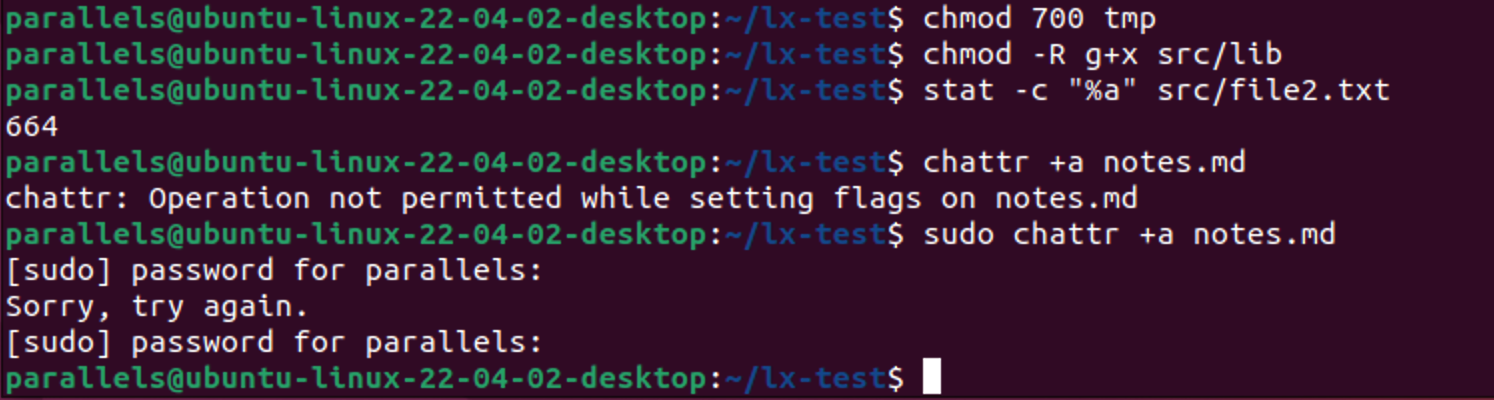
\includegraphics[width=0.8\textwidth]{linuxptD.png}
    \caption{Screenshot of Part D) Permissions and Ownership}
    \label{fig:problemsetD}
    
\end{figure}

\begin{figure}[h!]
    \centering
    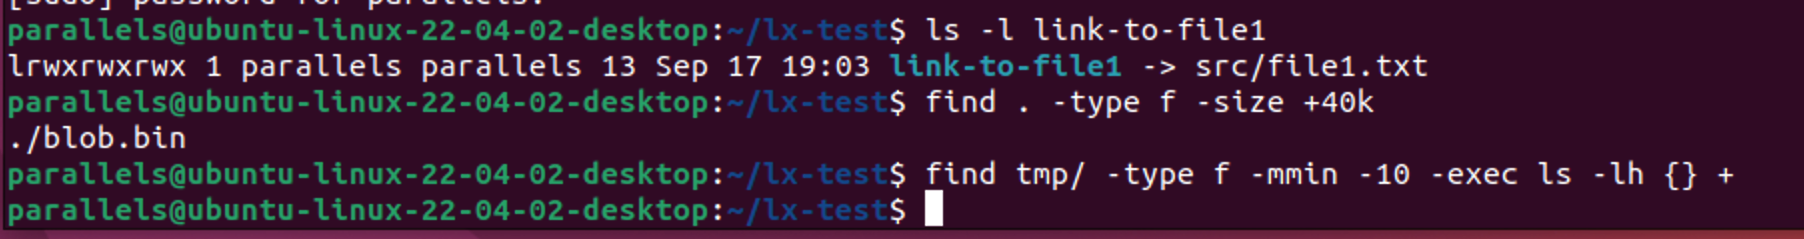
\includegraphics[width=0.8\textwidth]{linuxptE.png}
    \caption{Screenshot of Part E) Links and Find}
    \label{fig:problemsetE}
    
\end{figure}

\begin{figure}[h!]
    \centering
    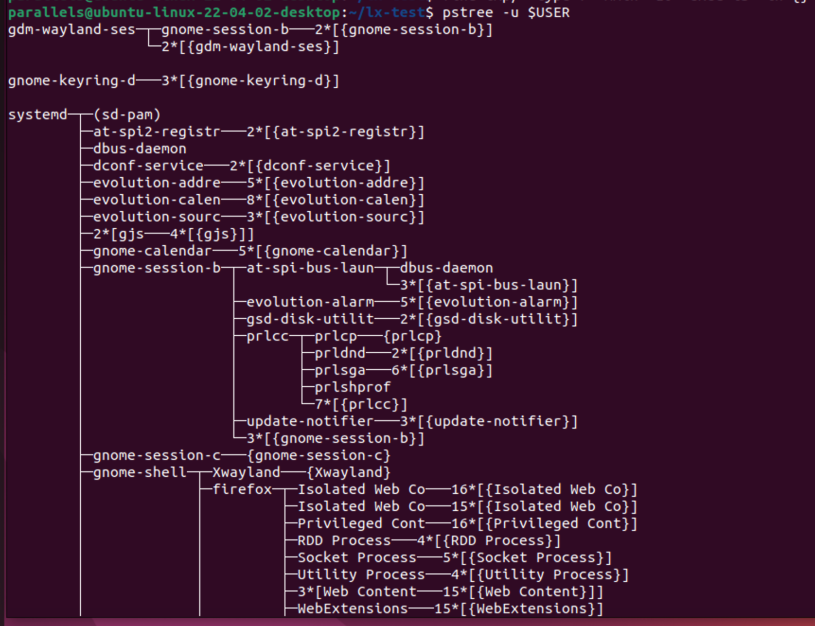
\includegraphics[width=0.8\textwidth]{linuxptF.png}
    \caption{Screenshot of the first part of Part F) Processes and Job Control}
    \label{fig:problemsetF}
    
\end{figure}

\begin{figure}[h!]
    \centering
    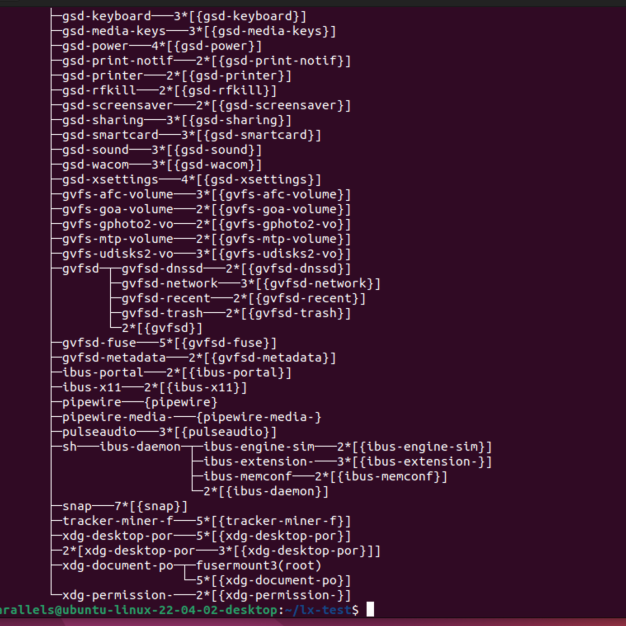
\includegraphics[width=0.8\textwidth]{linuxptF2.png}
    \caption{Screenshot of the second part of Part F) Processes and Job Control}
    \label{fig:problemsetEpt2}
    
\end{figure}

\begin{figure}[h!]
    \centering
    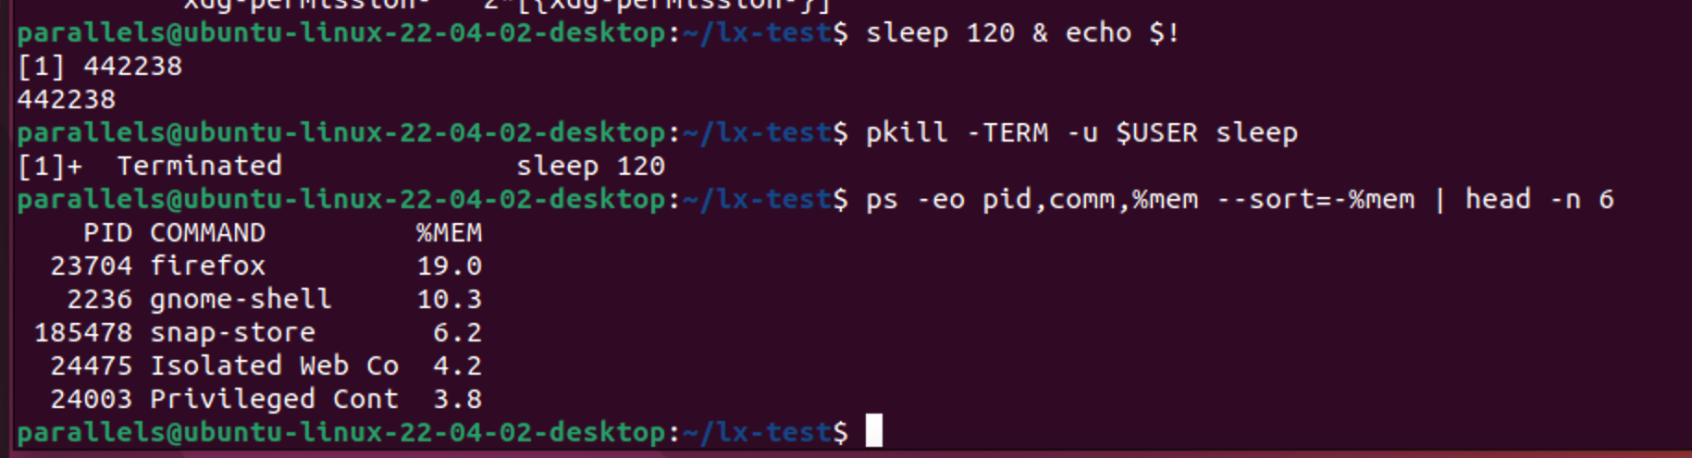
\includegraphics[width=0.8\textwidth]{linuxptF3.png}
    \caption{Screenshot of the third part of Part F) Processes and Job Control}
    \label{fig:problemsetFpt3}
    
\end{figure}

\begin{figure}[h!]
    \centering
    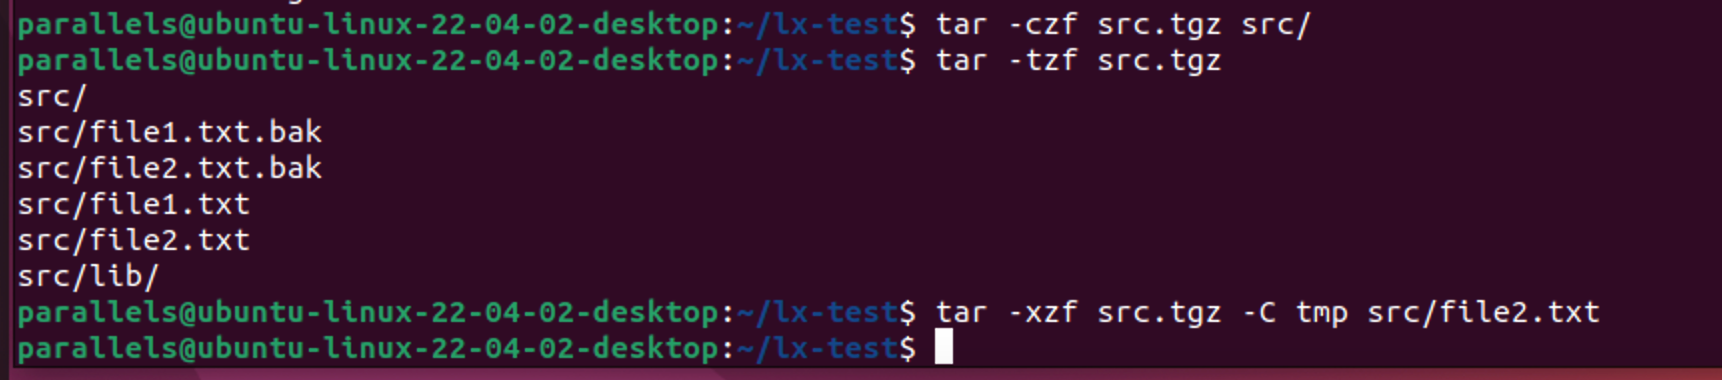
\includegraphics[width=0.8\textwidth]{linuxptG.png}
    \caption{Screenshot of Part G) Archiving and Compression}
    \label{fig:problemsetG}
    
\end{figure}

\begin{figure}[h!]
    \centering
    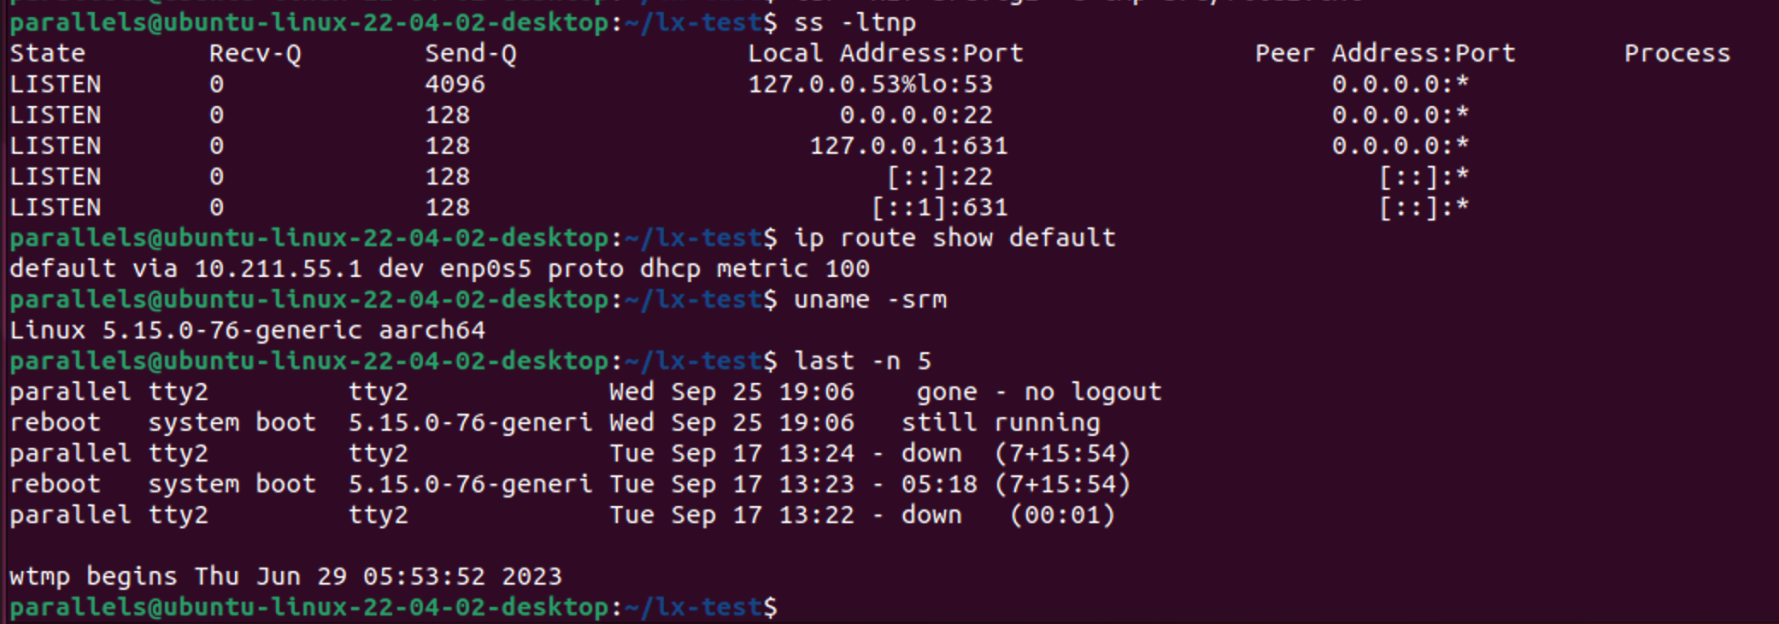
\includegraphics[width=0.8\textwidth]{linuxptH.png}
    \caption{Screenshot of Part H) Networking and System Info}
    \label{fig:problemsetH}
    
\end{figure}

\begin{figure}[h!]
    \centering
    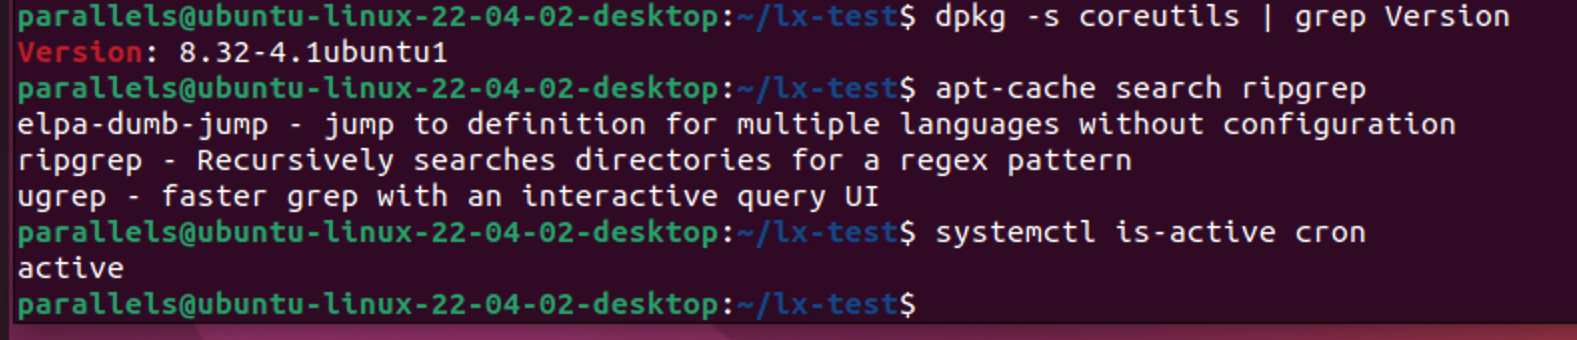
\includegraphics[width=0.8\textwidth]{linuxptI.png}
    \caption{Screenshot of Part I) Package and Services (Debian/Ubuntu)}
    \label{fig:problemsetI}
    
\end{figure}

\begin{figure}[h!]
    \centering
    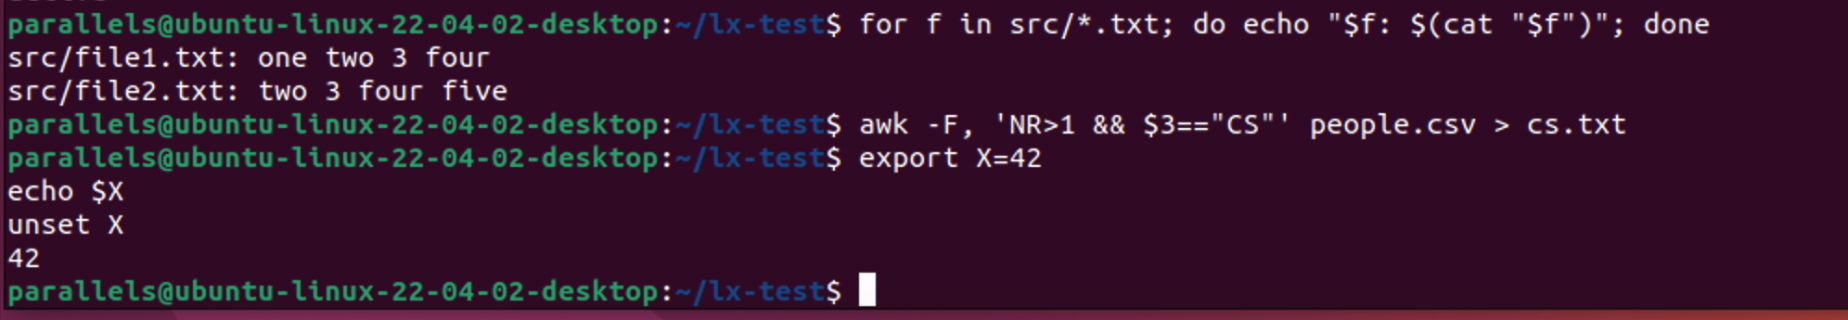
\includegraphics[width=0.8\textwidth]{linuxptJ.png}
    \caption{Screenshot of Part J) Bash and Scripting}
    \label{fig:problemsetJ}
    
\end{figure}
\chapter{Project Proposal \\
\small{\textit{-- Tamara Gonzalez Ibarra, Michelle Elias Flores, Sydney Winstead}}}
\index{Project Proposal} 
\index{Chapter!itProjectProposal}
\label{Chapter::itProjectProposal}

\section{Project Description}

Our group project for DevOps Principles and Practices is a web-based endless runner game called \textbf{Everscape}. The player controls a character that runs infinitely through a side-scrolling environment, avoiding increasingly challenging obstacles and collecting doubloons for bonus points. Users will compete for high scores, which will be securely stored in a backend database. Application security (e.g., preventing score tampering) and pipeline security (e.g., scanning Docker images) are a focus.

The project aims not only to deliver an engaging and aesthetically pleasing gaming experience but also to integrate DevSecOps practices throughout the development lifecycle.

\section{Sample Tasks}

\subsection*{Game Development}
\begin{itemize}
    \item Build the endless runner game logic, including jumping, collision detection, and scoring.
    \item Create a frontend interface for the player.
    \item Develop a backend service for storing scores.
\end{itemize}

\subsection*{DevSecOps Integration}
\begin{itemize}
    \item \textbf{Source Control}: Use GitHub for version control, pull requests, and branching.
    \item \textbf{Containerization}: Docker to containerize the frontend, backend, and database services.
    \item \textbf{Databases}: Deploy a lightweight containerized database (e.g., MySQL) for scores.
    \item \textbf{Testing}: Write unit tests (e.g., collision detection, score validation) and integration tests (e.g., API endpoints).
    \item \textbf{CI/CD Pipeline}: Set up GitHub Actions to build, test, and deploy containers automatically.
    \item \textbf{Hosting}: Deploy to a containerized environment (AWS ECS or Docker Compose locally).
\end{itemize}

\chapter{AWS Deployment \\
\small{\textit{-- Tamara Gonzalez Ibarra, Michelle Elias Flores, Sydney Winstead}}
\index{AWS Deployment} 
\index{Chapter!itAWSDeployment}
\label{Chapter::itAWSDeployment}}

\section{AWS Deployment Process}

To deploy our Dockerized website to AWS, we followed the steps outlined in Chapter~3, extending them with our own configuration and automation through a shell script. This section documents our full deployment workflow and provides the exact commands used, formatted with the \texttt{minted} package for clarity.

\subsection{Step 1: Install and Verify AWS CLI}

We first ensured that the AWS Command Line Interface (CLI) was installed and functioning properly on our machines. The CLI is required to authenticate, manage ECR repositories, and create App Runner services directly from the terminal.

\begin{minted}[fontsize=\small,breaklines]{bash}
# Verify that AWS CLI v2 is installed
aws --version
\end{minted}

If the command returned a version number such as \texttt{aws-cli/2.x.x}, we confirmed that AWS CLI was correctly installed.

\subsection{Step 2: Configure AWS SSO Credentials}

Next, we configured AWS Single Sign-On (SSO) to securely access our AWS account without using long-lived access keys. We initialized SSO configuration and created a profile named \texttt{docker-5}.

\begin{minted}[fontsize=\small,breaklines]{bash}
aws configure sso
# SSO session name: my-sso
# SSO start URL: https://d-90662881a4.awsapps.com/start
# SSO region: us-east-1
# Account: 846863293370
# Role: AdministratorAccess
# Default region: us-east-2
# Output format: json
# Profile name: docker-5
\end{minted}

After configuration, we authenticated using SSO:

\begin{minted}[fontsize=\small,breaklines]{bash}
aws sso login --profile docker-5
\end{minted}

This opened a browser window for login verification and returned a success message once authenticated.

\subsection{Step 3: Confirm AWS Credentials}

To ensure that our SSO credentials were valid and linked to the correct AWS account, we verified our caller identity.

\begin{minted}[fontsize=\small,breaklines]{bash}
aws sts get-caller-identity --profile docker-5
\end{minted}

This command returned the account ID, user ARN, and confirmed that our authentication was working correctly.

\subsection{Step 4: Set Environment Variables}

Before deploying, we set environment variables that define our AWS region, repository name, image tag, container port, and application name. These variables were later referenced by our deployment script.

\begin{minted}[fontsize=\small,breaklines]{bash}
export AWS_REGION="us-east-2"
export PROFILE="docker-5"
export ECR_REPO="my-app-repo"
export IMAGE_TAG="latest"
export CONTAINER_PORT=8080
export APP_NAME="my-apprunner-app"
export APP_ROLE_NAME="AppRunnerECRRole"
\end{minted}

\subsection{Step 5: Make the Deployment Script Executable}

We navigated to our project folder \texttt{color-buttons-app} and ensured that the deployment script had executable permissions.

\begin{minted}[fontsize=\small,breaklines]{bash}
cd Documents/color-buttons-app
chmod +x deploy.sh
\end{minted}

\subsection{Step 6: Deploy the Application to AWS}

Finally, we executed our \texttt{deploy.sh} script, which automated the following tasks:

\begin{enumerate}
    \item Creating or reusing an Amazon Elastic Container Registry (ECR) repository.
    \item Authenticating Docker to ECR using a short-lived token.
    \item Building, tagging, and pushing the Docker image to ECR.
    \item Creating or validating an IAM role for App Runner service access.
    \item Deploying the application to AWS App Runner.
    \item Continuously checking the service status until it became \texttt{RUNNING}.
\end{enumerate}

\begin{minted}[fontsize=\small,breaklines]{bash}
./deploy.sh
\end{minted}

The final output confirmed the public URL of our running service:

\begin{quote}
App Runner Service is running at: \url{https://8e4hdgaubu.us-east-2.awsapprunner.com/}
\end{quote}

\subsection{Step 7: Post-Deployment Verification}

After deployment, we tested the provided URL in a browser to ensure that the application loaded successfully and both buttons (blue and red) changed the background color as expected. This confirmed that our Docker image was correctly built, pushed, and deployed on AWS infrastructure.

\subsection{Step 8: Maintenance and Troubleshooting}

To verify future deployments or troubleshoot access, we used the following AWS CLI commands:

\begin{minted}[fontsize=\small,breaklines]{bash}
# List ECR repositories
aws ecr describe-repositories --region us-east-2 --profile docker-5

# Check App Runner service status
aws apprunner list-services --region us-east-2 --profile docker-5

# View service details
aws apprunner describe-service \
    --service-arn <SERVICE_ARN> \
    --region us-east-2 --profile docker-5
\end{minted}

These commands allowed us to monitor the health of our service and ensure that our web application remained accessible after deployment.
  
\subsection{UML Class Diagram Design}

\begin{figure}[h!]
    \centering
    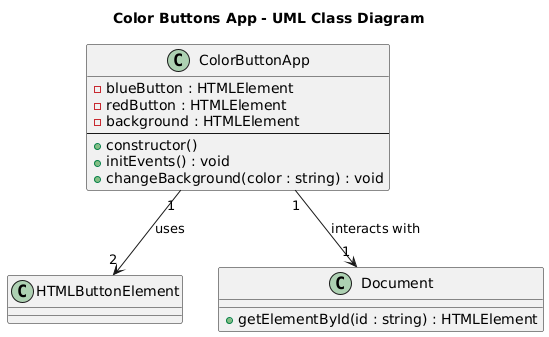
\includegraphics[width=0.8\textwidth]{png/ClassDiagram_Colorbutton.png}
    \caption{Class Diagram for updated class-based java script design}
    \label{fig:umlclassdiagram}
\end{figure}
\chapter{LaTeX Docker \\ 
\small{\textit{-- Tamara Gonzalez Ibarra, Michelle Elias Flores, Sydney Winstead}}}
\index{LaTeX Docker}
\index{Chapter!itLaTeXDocker}
\label{Chapter::itLaTeXDocker}

\section{Overview}

This chapter demonstrates how to create a minimal Docker container capable of compiling \LaTeX{} documents using \texttt{TeX Live}. This setup mimics how Overleaf performs compilations in isolated environments. Using Docker ensures reproducibility, portability, and isolation — essential for consistent document builds across different systems.

\section{Requirements}

Before proceeding, ensure Docker is installed and running:

\begin{minted}[fontsize=\small, bgcolor=lightgray!10]{bash}
docker --version
\end{minted}

You will also need a simple \LaTeX{} document to compile and a Dockerfile that defines the build environment.

\section{Minimal Project Structure}

We start with a simple directory structure (ASCII-safe):

\begin{minted}[fontsize=\small, bgcolor=lightgray!10]{text}
latex-docker/
|-- Dockerfile
`-- main.tex
\end{minted}

\section{The LaTeX Document}

Here is a minimal \texttt{main.tex} document (no \verb|\begin{document}| inside minted):

\begin{minted}[fontsize=\small, bgcolor=lightgray!10]{latex}
\documentclass{article}
\usepackage{lipsum}

\begin{document}

\section*{Hello from Docker \& TeX Live!}
\lipsum[1]

\end{document}
\end{minted}

\section{Dockerfile Explanation}

The Dockerfile defines the environment needed to build and compile the document:

\begin{minted}[fontsize=\small, bgcolor=lightgray!10]{docker}
# Use a minimal base image
FROM ubuntu:22.04

# Set noninteractive mode for installation
ENV DEBIAN_FRONTEND=noninteractive

# Install TeX Live packages
RUN apt-get update && \
    apt-get install -y --no-install-recommends \
        texlive-latex-base \
        texlive-latex-recommended \
        texlive-latex-extra \
        texlive-fonts-recommended \
        latexmk && \
    apt-get clean && \
    rm -rf /var/lib/apt/lists/*

# Set the working directory
WORKDIR /data

# Command to compile LaTeX documents
ENTRYPOINT ["latexmk", "-pdf", "-interaction=nonstopmode"]
\end{minted}

\section{Building the Docker Image}

Build the image from the same directory as your Dockerfile:

\begin{minted}[fontsize=\small, bgcolor=lightgray!10]{bash}
docker build -t latex-docker .
\end{minted}

This creates a Docker image named \texttt{latex-docker} with all dependencies to compile \LaTeX{} documents.

\section{Compiling the Document}

Compile your document by mounting the current directory:

\begin{minted}[fontsize=\small, bgcolor=lightgray!10]{bash}
docker run --rm -v $(pwd):/data latex-docker main.tex
\end{minted}

After execution, you should find a compiled \texttt{main.pdf} in your directory.

\section{Conclusion}

Using Docker with TeX Live provides a reproducible and portable environment for \LaTeX{} compilation. This mirrors Overleaf's backend concept: isolated container environments ensure consistent, dependency-free builds across systems.

\chapter{Bugzilla Docker}
\label{Chapter::itBugzillaDocker}
\index{itBugzillaDocker}
\index{Chapter!itBugzillaDocker}

\begin{flushleft}
\small{\textit{-- Tamara Gonzalez Ibarra, Sydney Winstead, Michelle Elias Flores}}
\end{flushleft}

\section{Overview}
This report outlines the process of setting up a \textbf{Bugzilla Docker container} on a DigitalOcean droplet. The setup included creating a droplet with Docker preinstalled, connecting via SSH, configuring Bugzilla using Docker Compose, and verifying that the Bugzilla instance was running successfully.

\section{DigitalOcean Droplet Configuration}

A new DigitalOcean droplet was created using the official \textbf{Docker 1-Click App}.  
After creation, we set up an SSH key for secure access and connected using:

\begin{minted}[fontsize=\small, bgcolor=gray!5, linenos]{bash}
ssh root@167.99.121.94
\end{minted}

Upon connection, the system displayed:

\begin{quote}
Welcome to DigitalOcean's 1-Click Docker Droplet.  
To keep this Droplet secure, the UFW firewall is enabled.  
All ports are BLOCKED except 22 (SSH), 2375 (Docker) and 2376 (Docker).
\end{quote}

To confirm Docker installation:

\begin{minted}[fontsize=\small, bgcolor=gray!5, linenos]{bash}
docker --version
\end{minted}

\section{Bugzilla Setup and Configuration}

We created and edited a Docker Compose file at \texttt{/opt/bugzilla/docker-compose.yml}:

\begin{minted}[fontsize=\small, bgcolor=gray!5, linenos]{yaml}
services:
  db:
    image: mariadb:10.5
    container_name: bugzilla_db
    restart: always
    environment:
      MYSQL_ROOT_PASSWORD: rootpassword
      MYSQL_DATABASE: bugzilla
      MYSQL_USER: bugzilla
      MYSQL_PASSWORD: bugzilla123
    volumes:
      - db_data:/var/lib/mysql

  bugzilla:
    image: bugzilla/bugzilla-dev
    container_name: bugzilla_app
    restart: always
    depends_on:
      - db
    ports:
      - "80:80"
    environment:
      DB_HOST: db
      DB_DATABASE: bugzilla
      DB_USER: bugzilla
      DB_PASSWORD: bugzilla123
    volumes:
      - bugzilla_data:/var/www/html

volumes:
  db_data:
  bugzilla_data:
\end{minted}

Once configured, we started both services:

\begin{minted}[fontsize=\small, bgcolor=gray!5, linenos]{bash}
docker compose up -d
docker compose ps
\end{minted}

\section{Verification}

After successful startup, Bugzilla was accessible at:

\begin{quote}
\url{http://167.99.121.94/}
\end{quote}

We verified that both the \texttt{bugzilla\_app} and \texttt{bugzilla\_db} containers were active and persistent upon restart.

Bugzilla was successfully deployed via Docker Compose using a MariaDB backend.  
The instance is reachable publicly at port 80 and functions as expected.

\chapter{Overleaf Docker \\
\small{\textit{-- Tamara Gonzalez Ibarra, Michelle Elias Flores, Sydney Winstead}}
\index{itOverleafDocker} 
\index{Chapter!itOverleafDocker}
\label{Chapter::itOverleafDocker}}

\section{Overview}
This report details the process of deploying an \textbf{Overleaf Docker container} on DigitalOcean.  
The deployment reused the same droplet and exposed Overleaf through port 3000 with a MongoDB backend.

\section{Droplet Connection and Setup}

We connected to our existing droplet via SSH:
\begin{minted}[fontsize=\small, bgcolor=gray!5, linenos]{bash}
ssh root@167.99.121.94
\end{minted}

Then we created a dedicated Overleaf directory:
\begin{minted}[fontsize=\small, bgcolor=gray!5, linenos]{bash}
mkdir -p /opt/overleaf
cd /opt/overleaf
\end{minted}

\section{Docker Compose Configuration}

We then created a new \texttt{docker-compose.yml} file:
\begin{minted}[fontsize=\small, bgcolor=gray!5, linenos]{yaml}
version: '3'

services:
  db:
    image: mongo:4.4
    container_name: overleaf-db
    restart: always
    volumes:
      - db_data:/data/db

  overleaf:
    image: overleaf/overleaf:latest
    container_name: overleaf
    restart: always
    ports:
      - "3000:80"
    environment:
      - MONGO_URL=mongodb://db:27017/overleaf
      - ROOT_URL=http://167.99.121.94:3000

volumes:
  db_data:
\end{minted}

After saving, we launched the service:
\begin{minted}[fontsize=\small, bgcolor=gray!5, linenos]{bash}
docker-compose up -d
\end{minted}

\section{Verification}
Once running, we confirmed Overleaf was accessible at:
\begin{quote}
\url{http://167.99.121.94:3000/}
\end{quote}

We confirmed both containers were up and communicating correctly using:
\begin{minted}[fontsize=\small, bgcolor=gray!5, linenos]{bash}
docker ps
\end{minted}
\chapter{Domain Names, SSL, and Versioning}
\label{Chapter::itDomainNames}
\index{itDomainNames}
\index{Chapter!itDomainNames}

\begin{flushleft}
\small{\textit{-- Tamara Gonzalez Ibarra, Michelle Elias Flores, Sydney Winstead}}
\end{flushleft}




\appendix
\chapter{Appendix \\
\small{\textit{-- Tamara Gonzalez Ibarra}}
\index{appendix} 
\index{Chapter!Appendix}
\label{Chapter::Appendix}}

% makeglossaries dsnManual -- from command prompt.
\clearpage
%\printglossaries


\printnoidxglossaries

\bibliography{bibfile}
%\bibliographystyle{unsrt}
\bibliographystyle{IEEEtran}

\printindex
%\input{dsnManual.idx}
\end{document}
